\subsection{OSM Results}
The \ref{fig:cirroscase1180-cpu}, \ref{fig:cirroscase1180-mem} and \ref{fig:osm-top-3-lifecycle} shows the CPU utilization, memory utilization and CPU utilization throught the life cycle of the experiment respectively. Let us consider the important dockers in each case and list their functionalities to realize why they have consumed maximum CPU.

\subsubsection{CPU utilization}

The \ref{fig:cirroscase1180-cpu} shows CPU utilization. The first 5 OSM dockers are:

\begin{itemize}
	\item \textbf{osm\_ro:} This is the Resource Orchestrator for OSM. 
	The resource orchestrator is responsible for co-ordinating resource allocation across multiple geo-distributed VIM types.
	It is responsible in processing the resource-allocation requirements of the VNF as per parts of the VNFD and driving the VIM to allocate appropriate compute, network, and storage resources for the deployment of VNFs with their interconnection. 
	
	\item \textbf{osm\_lcm:} This is the Life Cycle Management module for OSM. 
	This docker is responsible for set of operations related to the life cycle of a VNF and NS
	
	\begin{itemize}
		\item \textit{NS LCM operations:} 
		1) On-board Network Service
		2) Instantiate Network Service
		3) Scale Network Service
		4) Update Network Service by supporting Network Service configuration changes
		Create, delete, query, and update of VNFFGs associated to a Network Service.
		5) Terminate Network Services
		
		\item \textit{VNF LCM operations:} 1) Instantiate VNF (create a VNF using the VNF on-boarding artefacts)
		2) Scale VNF (increase or reduce the capacity of the VNF).
		3) Update and/or Upgrade VNF (support VNF software and/or configuration changes of various complexity).
		4) Terminate VNF (release VNF-associated NFVI resources and return it to NFVI resource pool)
	\end{itemize}
	
	
	
	\item \textbf{osm\_mon:} This is the monitoring module for OSM. 
	The main task of this docker is to retreive metrics from VIM. 
	It keeps polling VIM every 30 seconds. 
	
	\item \textbf{osm\_ro\_db:} This is called RO database module.
	RO module in OSM maintains its own database called ro-db. (RO module is usually edited to enable or disable this particular module)
	This module takes care of database related operations. According to the osm/ro.git, ro-db stores different IDs like vnfd id ,osm id, tenant id, vim id etc. There is something called scenario. ro db stores these scenarios and scenario ID and then a scenario gets executed when the scenario id matches with the right tenant id, osm id and vnfd id. 
	It stores vim actions, wim actions and they are processed sequentially. 
	
	\item \textbf{osm\_nbi:} North Bound Interface of OSM. Restful server that follows ETSI SOL005 interface.
	It is the unique entry point for all the interactions with the OSS/UI system.
	This serves as the interface for MANO operations.
	(OSM's NBI offers all the necessary abstractions to allow clients for the complete control, operation and supervision od the NS.)
\end{itemize}

\begin{figure}[h]
	\centering
	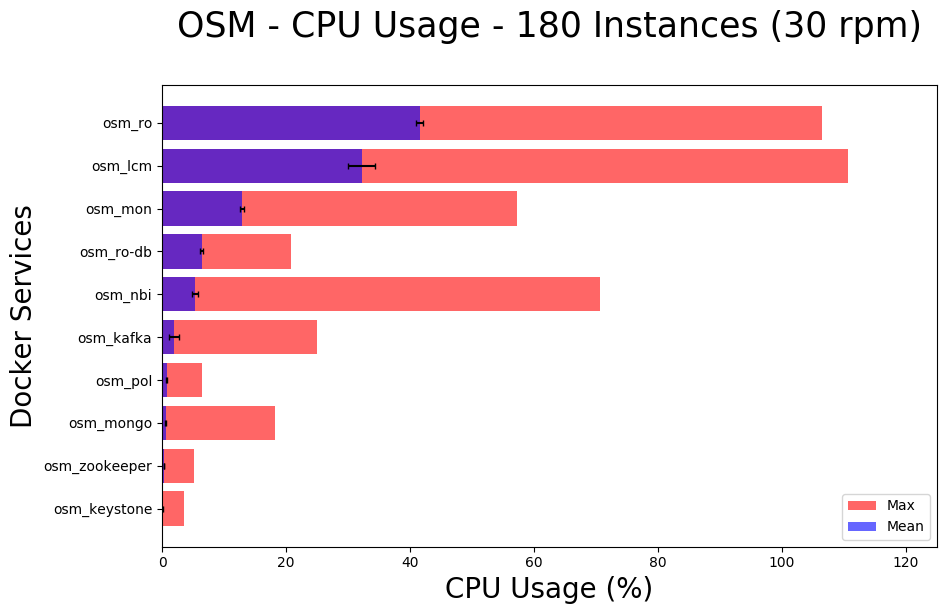
\includegraphics[width=1\linewidth]{../figures/scalability_graphs/Horizontal-Docker-Graphs/osm/cirros_case1_180-CPU}
	\caption{OSM CPU}
	\label{fig:cirroscase1180-cpu}
\end{figure}

\pagebreak



\subsubsection{Memory Utilization}

The first 5 OSM dockers in memory utilization graph are:

\begin{itemize}
	\item \textbf{osm\_mongo:} This is a common non relational database for OSM modules.
	\item \textbf{osm\_kafka:} This module provides a Kafka bus used for OSM communication.
	\item \textbf{osm\_nbi:} This is the north bound interface for OSM module. The functionalities of this module remains the same(as explained in the previous subsection)
	
	\item \textbf{osm\_light-ui:} This docker is an implementation of a web GUI to interact with the Northbound API. (The framework allows editing, validating, visualizing the descriptors of services and components both textually and graphically)
	\item \textbf{osm\_ro\_db:} This is the RO database. The functionalities of this module remains the same (as explained in the previous subsection)
	
\end{itemize}



\begin{figure}[h]
	\centering
	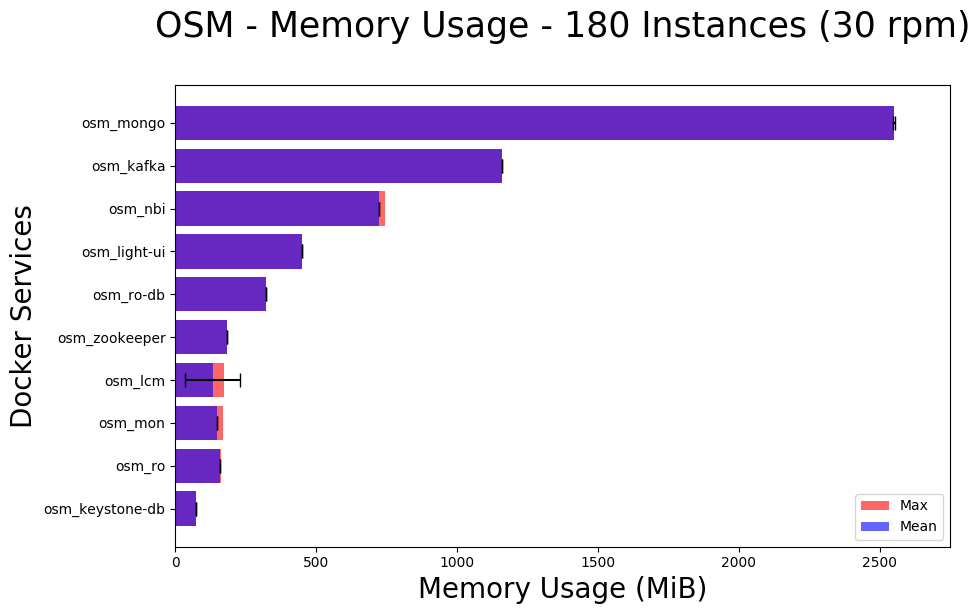
\includegraphics[width=1\linewidth]{../figures/scalability_graphs/Horizontal-Docker-Graphs/osm/cirros_case1_180-MEM}
	\caption{OSM MEM}
	\label{fig:cirroscase1180-mem}
\end{figure}


\subsubsection{Lifecycle}

We now have the life cycle graphs of the entire experiment. This shows the distribution of the CPU usage among the top 3 dockers throughout the experiment. The experiment lasted for about 10 minutes.

We can observe that the ro module of OSM got continuous requests over the time and at the end all the termination requests came at once. Also LCM , mon modules continously processed the requests. mon module retrieved metric information continuously and the same trend
remains throughout the experiment.

\begin{figure}[h]
	\centering
	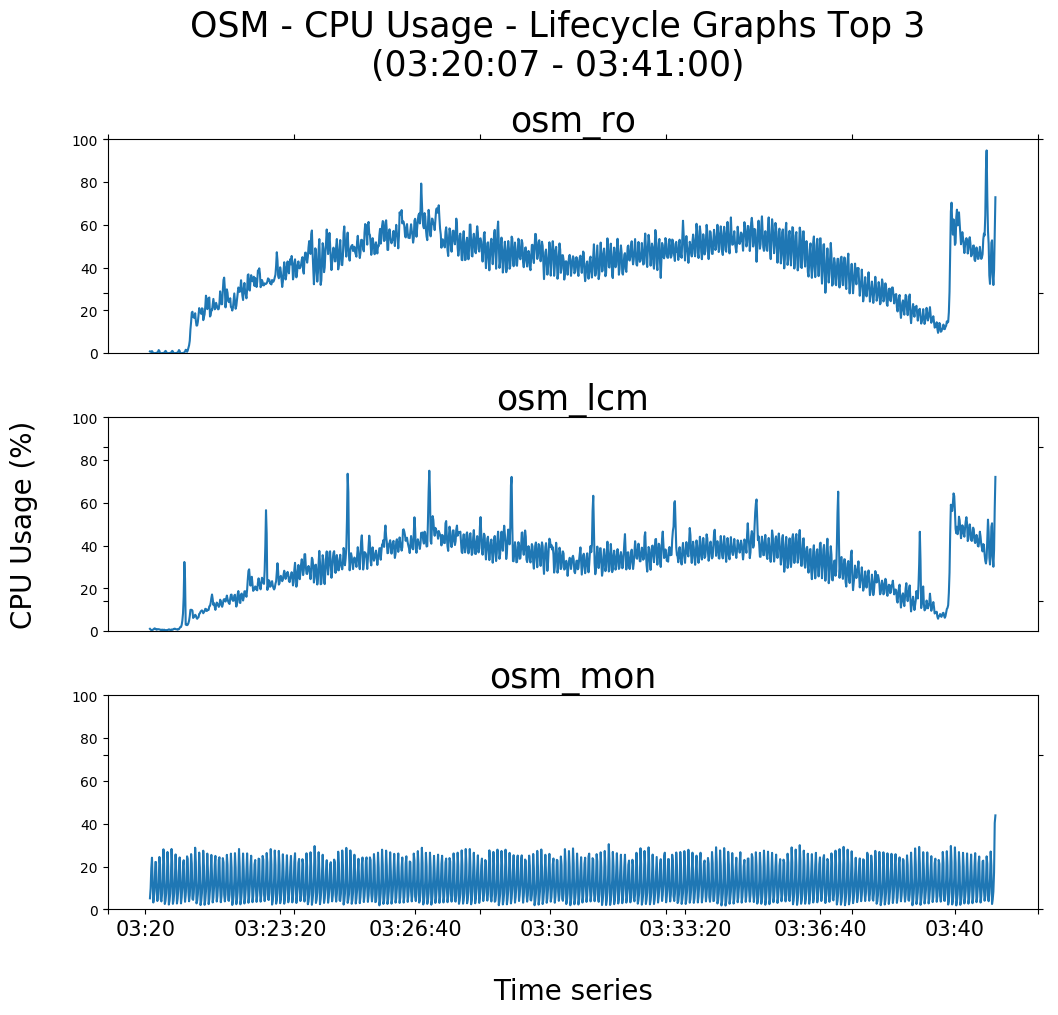
\includegraphics[width=1\linewidth]{figures/scalability_graphs/Lifecycle-Graphs-Top-3/OSM-TOP-3-Lifecycle}
	\caption{OSM LS}
	\label{fig:osm-top-3-lifecycle}
\end{figure}
